\section{Verification Runtime}
Support for \texttt{async}, \texttt{finish}, \texttt{isolated}, and \texttt{future} is handled by 4 main classes in VR, \texttt{Activity}, \texttt{Place}, \texttt{Future}, and \texttt{DataRaceDetector}. 

\texttt{Activity}, inherits from Java's \texttt{Thread} class, and is used to represent each HJ task. Each \texttt{Activity} contains a reference to its parent and children tasks, a reference to a \texttt{Future} object, and methods to support the finish keyword. When an \texttt{Activity} is created the compiler inserts the computation associated with the \texttt{Activity} into its \texttt{runHjTask} method. \figref{fig:hello-world} shows how this works for a simple HJ program.

\begin{figure}[t]
\begin{center}
{\small
\begin{verbatim}
public class Foo {
    public static void main(String[] argv) {
        async {
            System.out.println("Hello World");}}}

public class Foo {
    public static void main(String[] paramArrayOfString) {
        place threadPool = Runtime.here();
        Activity childTask = new FooAsync();
        threadPool.runAsync(childTask);}}

class FooAsync extends Activity {
    // HJ task code
    public void runHjTask() {
        System.out.println("Hello World");}}
\end{verbatim}
}
\end{center}
\vspace{-10pt}
\caption{HJ Compiled "Hello World" program.}
\label{fig:hello-world}
\end{figure}

In HJ, all tasks created within a finish statement (including nested async statements) must complete before the parent task may proceed beyond the scope of the finish statement. In VR, the references in the \texttt{Activity} class are used to maintain this hierarchy. When an \texttt{Activity} is created via \texttt{async} keyword inside of a finish statement then it is given a reference to the \texttt{Activity} that created it and vice versa. If the child task terminates it passes its children to its parent performing an operation called task adoption. When the parent activity reaches the end of a finish statement it performs a join on all of its children including those received via adoption. 

Activities can also be created using {\tt final future<T> f = async<T> Expr;}. Whenever a \texttt{future} keyword is encountered VR creates an \texttt{Activity} that returns a \texttt{Future} upon termination. VR uses \texttt{java.util.Concurrent.CountDown}-\texttt{latch} to handle the synchronization between the task that creates the future (producer) and the task that requests it (consumer). \figref{fig:futures} contains methods that show how communication between consumers and the producer is handled. The producer creates and obtains the lock upon construction. When the producer has completed all of its computation and is ready to terminate it calls \texttt{setFuture} releasing the lock. This allows consumers access to the data upon all subsequent \texttt{get} calls.

\begin{figure}[t]
\begin{center}
{\small
\begin{verbatim}
	//Consumer    
	public java.lang.Object get() {        
        //Exception handling omitted
        lock.await();
        return item;}
	//Producer 
    public void setFuture(java.lang.Object object) {        
        item = object;
        lock.countDown();}
\end{verbatim}
}
\end{center}
\caption{The operation of Futures within VR.}
\label{fig:futures}
\end{figure} 

The \texttt{isolated} keyword is handled outside of the \texttt{Activity} class. VR uses a single global lock, contained within the \texttt{Place} class, to enforce mutual exclusion between isolated statements. In the HJ language there are two different forms of isolated statements {\tt isolated}~$\langle${\it stmt1}$\rangle$ and {\tt isolated(Obj 1, Obj 2, ..., Obj n)}~$\langle${\it stmt1}$\rangle$ where the second form refines isolation to cover only the specified objects whilst the first form isolates all objects contained within its scope. However, in VR all isolated statements are treated as the first form. This provides the same answer in terms of correctness, but is potentially less efficient than the semantics provide.

In summary, the architecture of VR is for the most part distributed amongst 4 classes. The user calls \texttt{DataRaceDetector}, the driver of the runtime, which in turn runs the HJ program the user specified. Every task is given its own thread, and each thread has variables specific to what its properties are, whether a future or an async task. Every thread also has a link to the thread that created it, and threads it created, which is used for finish statements. The isolated lock is global, and the thread that holds the lock is responsible for releasing it when it is finished. \figref{fig:codeHierarchy} shows an abstract overview of the code sample in \figref{fig:sampleCode}.

\begin{figure}[t]
\begin{center}
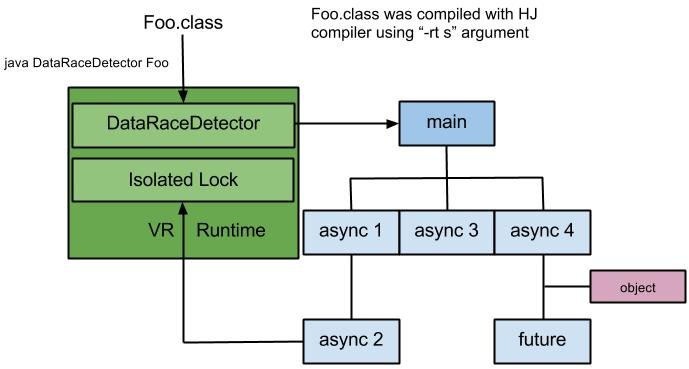
\includegraphics[width=3.25in]{../figs/CodeHierarchy}
\end{center}
\vspace{-10pt}
\caption{The VR execution and architecture.}
\label{fig:codeHierarchy}
\end{figure}

\begin{figure}
\begin{center}
{\small
\begin{verbatim}
public class Foo {
    public static void main(String args[]) {
        finish {
            async { // async 1
                async isolated <stmt> //async 2}
            async ; // async 3
            async { // async 4
                final future<Object> object = 
                async<Object>{return object};
                object.get(); }}}}
\end{verbatim}
}
\end{center}
\caption{A simple code sample.}
\label{fig:sampleCode}
\end{figure}

VR operates independent of JPF, but is obviously best suited within JPF because of the potentially large number of threads it creates. In all VR is composed of 12 Java classes and 992 lines of code. This small design is inherently much simpler than HJ which is composed of more that 100 Java classes and >10,000 lines of code. The small design also simplifies the interaction with JPF. The repository for VR can be found at \texttt{https://bitbucket.org/bchase524/jpf-hj}.



